\chapter{Background and Technologies}
\label{sec:background}

This chapter provides a comprehensive overview of the core concepts and technologies underpinning the project. It begins by exploring the architectural shift from traditional monolithic systems to decentralized microservices, then moving to the main differences between imperative and reactive programming models, highlighting how the latter addresses the high-concurrency demands of modern cloud infrastructure.

Furthermore, it examines the project's technological stack and the different communication paradigms adopted to allow the system's components to interact with each other.

%%%%%%%%%%%%%%%%%%%%%%%%%%%%%%%%%%%%%%
%%% 2.1 Microservices Architecture %%%
%%%%%%%%%%%%%%%%%%%%%%%%%%%%%%%%%%%%%%

\section{Microservices Architecture}
\label{sec:microservices}

The evolution of cloud computing has fundamentally altered how enterprise applications are designed, developed, and maintained. While monolithic architectures served as the industry standard for decades, they present significant scaling and maintenance limitations as systems grow in complexity. To address these bottlenecks, the software industry has increasingly adopted the microservices architecture, a paradigm that decomposes large, rigid applications into a suite of smaller, independent services \cite{aws_microservices}.

\subsection{Principles of Microservices}

Unlike a monolithic application that shares a single massive codebase and a centralized database, a microservices architecture is built upon the principle of decentralization and loose coupling. Each microservice is designed around a specific business capability or "bounded context" \cite{microsoft_microservices}. For example, in an e-commerce platform like Smart Travel, the catalog management and the order processing capabilities are handled by distinct autonomous services.

The foundational principles of this architecture include:
\begin{itemize}
    \item \textbf{Autonomy and Independent Deployment:} Each service is a self-contained unit. It encapsulates its own code, dependencies, and typically its own data store. This allows teams to update, deploy, and scale a single service without needing to recompile or redeploy the entire system.
    \item \textbf{Lightweight Communication:} Because microservices operate as independent processes, they must communicate over a network to fulfill complex business transactions. This is achieved using well-defined \textit{Application Programming Interfaces} (\gls{API}s), typically relying on synchronous protocols like HTTP or asynchronous message delivery mechanisms.
    \item \textbf{Decentralized Data Management:} Rather than relying on a single shared database schema, each microservice manages its own database, choosing the \gls{DBMS} technology best suited to its specific data access patterns.
\end{itemize}
 
\begin{figure}[ht]
	\centering
    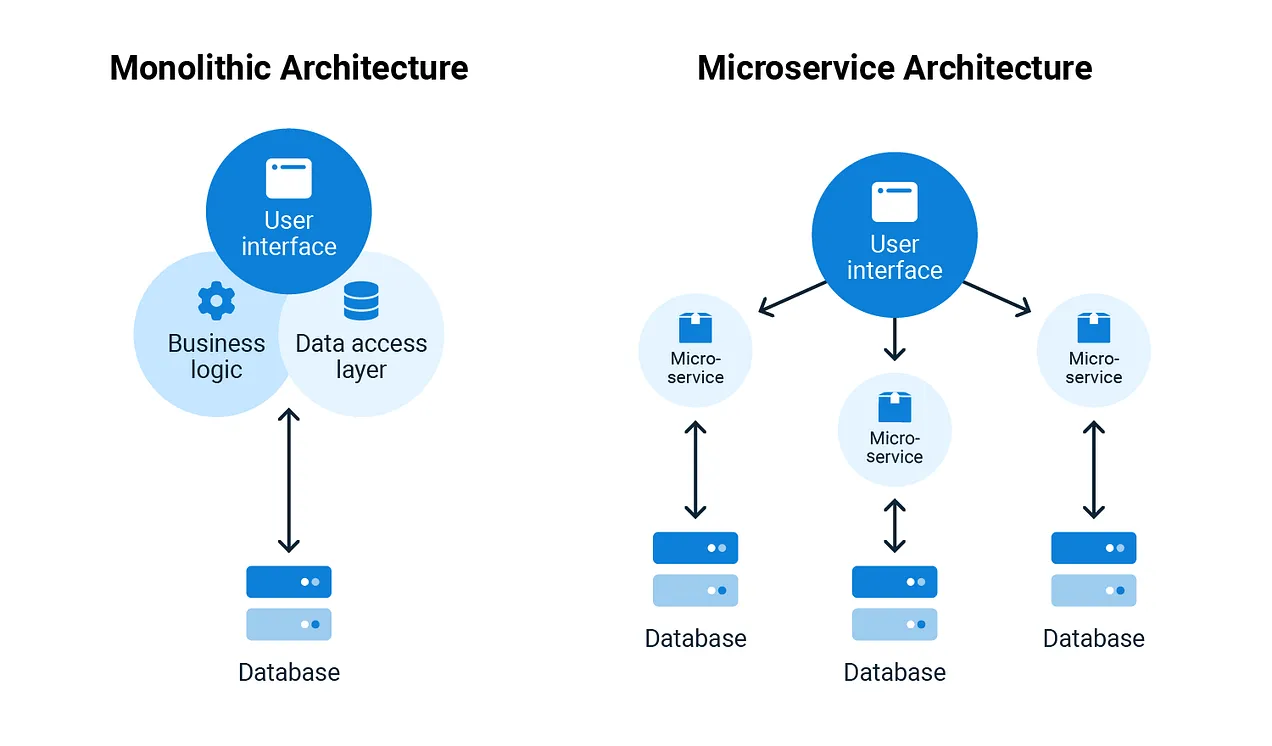
\includegraphics[width=\textwidth]{images/ch1/1_monolith-vs-microservices.png}
	\caption[Monolithic vs. Microservices architecture]{Monolithic vs. Microservices architecture. \textit{Source: \cite{coderco_monoliths_vs_microservices}}}
    \label{fig:monolith_vs_microservices}
\end{figure}

\subsection{Benefits}

The shift from monolithic to microservices architecture provides several advantages \cite{tayoolaigbe_microservices}:

\begin{itemize}
    \item \textbf{Targeted Scalability:} In a monolithic system, an unexpected spike in traffic for one specific feature (e.g., the payment gateway) requires scaling the entire application, leading to resource wastage. Microservices allow infrastructure teams to scale only the specific services experiencing high demand, optimizing cloud resource consumption and costs.
    \item \textbf{Fault Isolation and Resilience:} Because microservices are loosely coupled, a critical bug, memory leak, or crash in one service does not inherently cascade and bring down the entire platform. The application can handle partial failures gracefully, degrading functionality while keeping core operations online.
    \item \textbf{Technological Freedom:} Teams are not locked into a single technology stack. Since microservices communicate via standardized network protocols, developers can select the most appropriate programming language, framework, and database for each specific task. This flexibility allowed the Smart Travel project to implement and compare different Java frameworks (Spring Boot and Quarkus) within the same ecosystem.
    \item \textbf{Agility and CI/CD:} Smaller codebases are easier to understand, test, and deploy. This structure naturally complements DevOps practices, enabling \gls{CI/CD} pipelines to push frequent updates to production.
\end{itemize}

\subsection{Challenges and Limitations}

Despite its significant advantages, adopting a microservices architecture introduces a high degree of distributed system complexity. Some of the key challenges include:

\begin{itemize}
    \item \textbf{Operational Overhead and Monitoring:} Managing dozens of independently running services is inherently more complex than managing a single monolith. It requires sophisticated container orchestration platforms (such as Kubernetes or OKD) and centralized observability tools for distributed tracing, log aggregation, and metric monitoring to identify where a failure occurred across the network.
    \item \textbf{Network Latency and Congestion:} Replacing in-memory function calls with remote network requests introduces latency. If a single user action requires a long chain of inter-service API calls, the accumulated network overhead can severely degrade system performance.
    \item \textbf{Data Consistency:} Because each service maintains its own database, achieving data consistency across the system becomes a major challenge. Traditional \texttt{\gls{ACID}} transactions that span multiple tables are no longer feasible. Instead, developers must rely on complex distributed transaction patterns and embrace \textit{eventual consistency}.
\end{itemize}

2.2 Programming Paradigms: Imperative vs. Reactive programming models.

2.3 Event-Driven Architecture: Asynchronous communication and message brokers (focus on RabbitMQ).

2.4 Backend Technologies: Spring Boot and Quarkus

2.5 Frontend Technologies: Single Page Applications (SPA), Angular, RxJS, and PrimeNG.

2.6 Database Technologies: NoSQL concepts and MongoDB.

2.7 API Paradigms: REST vs. GraphQL.